\documentclass[12pt,twoside]{book}
\usepackage[utf8]{inputenc}
\usepackage[export]{adjustbox}
\usepackage[a4paper, top=25mm, bottom=25mm, inner=20mm, outer=30mm]{geometry}
\usepackage{afterpage,blindtext,color,hyperref,ragged2e,graphicx,fancyhdr}
\usepackage[dvipsnames]{xcolor}
\usepackage{newtxtext}
\usepackage{xcolor}
\usepackage{xspace}
\usepackage[explicit]{titlesec}
\usepackage{lipsum, caption}
\usepackage{type1cm}
\usepackage[nopostdot,toc,acronym,nomain,nonumberlist]{glossaries}
\usepackage[backend=biber,style=numeric-comp
,sorting=none]{biblatex}
\addbibresource{references.bib}
\usepackage{multirow}
\usepackage{mfirstuc}
\newcommand{\ssc}[1]{\textsc{\capitalisewords{\MakeLowercase{#1}}}}
\newcommand{\asc}[1]{\textsc{{\MakeLowercase{#1}}}}
\usepackage{pdfpages}
\usepackage{bbold}
\usepackage[title]{appendix}
\usepackage{slashed}
\usepackage{datetime}
\usepackage{graphicx}
\usepackage{amsmath,bm,amsfonts}
\usepackage[]{mdframed}
\usepackage{adjustbox}
\usepackage{hyperref}
\usepackage{tabu}
\usepackage{tabularray}
\usepackage[most]{tcolorbox}
\usepackage{tocloft}  % for lists for custom environments
\usepackage{xparse}
\usepackage{quotes}

\NewTblrTheme{longtable1}{
    \DefTblrTemplate{conthead-text}{fancy}{}
        \SetTblrTemplate{conthead-text}{fancy}

    \DefTblrTemplate{contfoot-text}{fancy}{[Continue on next page]}
        \SetTblrTemplate{contfoot-text}{fancy}

    \DefTblrTemplate{caption}{default}{
        \UseTblrTemplate{caption-tag}{default}
        \UseTblrTemplate{caption-sep}{default}
        \UseTblrTemplate{caption-text}{default}
        }
    \DefTblrTemplate{capcont}{default}{
        \UseTblrTemplate{caption-tag}{}
        \UseTblrTemplate{caption-sep}{}
        \UseTblrTemplate{caption-text}{}
        \UseTblrTemplate{conthead-text}{}
        }}

\newdateformat{monthyeardate}{%
  \monthname[\THEMONTH], \THEYEAR}

\titlespacing{\section}{0pt}{0pt}{0pt}
\titlespacing{\subsection}{0pt}{0pt}{0pt}

%\makeatletter
%\def\ttl@mkchap@i#1#2#3#4#5#6#7{%
%    \ttl@assign\@tempskipa#3\relax\beforetitleunit
%    \vspace{\@tempskipa}%<<<<<< REMOVE THE * AFTER \vspace
%    \global\@afterindenttrue
%    \ifcase#5 \global\@afterindentfalse\fi
%    \ttl@assign\@tempskipb#4\relax\aftertitleunit
%    \ttl@topmode{\@tempskipb}{%
%        \ttl@select{#6}{#1}{#2}{#7}}%
%    \ttl@finmarks  % Outside the box!
%    \@ifundefined{ttlp@#6}{}{\ttlp@write{#6}}}
%\makeatother
%
%\renewcommand{\chaptermark}[1]{\markboth{{\chaptername\ \thechapter.\ #1}}{}}
% Following line generates undefined control sequence: section for me, so comment it out for now
%\renewcommand{\sectionmark}[1]{\markright{{\sectionname\ \thesection.\ #1}}{}}


\newcommand*\NewPage{\newpage\null\thispagestyle{empty}\newpage}

\setlength{\parskip}{0.6em}
\setlength{\parindent}{20pt}
\graphicspath{{images/}}
\definecolor{gray75}{gray}{0.75}
\newcommand{\hsp}{\hspace{20pt}}
\hypersetup{colorlinks=false,linktoc=all, linkcolor=LimeGreen}

\pagestyle{fancy}
\fancyhf{}
\fancyhead[LE]{\leftmark}
\fancyhead[RO]{\rightmark}
\fancyfoot[LE,RO]{\thepage}

\titleformat{\title}[display]
  {\flushright\normalfont\fontsize{50}{}\sffamily\bfseries}
  {\sffamily\fontsize{50}{50}\textbf{\textcolor{LimeGreen}{{\partname}~\thetitle\vskip40pt}}}{0pt}
  {\textcolor{LimeGreen}{\fontsize{40}{0}{#1}\vskip10pt}\titlespacing*{\part}{0pt}{-1pt}{0pt}}

\titleformat{\part}[display]
  {\flushleft\normalfont\fontsize{50}{}\sffamily\bfseries}
  {\sffamily\fontsize{80}{50}\textbf{\textcolor{LimeGreen}{{\partname}~\thepart\vskip40pt}}}{0pt}
  {\textcolor{LimeGreen}{\fontsize{40}{10}{#1}\vskip10pt}\titlespacing*{\part}{0pt}{0pt}{0pt}}


\titleformat{\chapter}[display]
  {\normalfont\Huge\sffamily\bfseries}
  {\sffamily\flushright\fontsize{70}{0}\textbf{\textcolor{LimeGreen}{{\Huge\chaptername}~\thechapter\vskip0pt\rule{\textwidth}{5pt}}}}{0pt}
  {\flushleft\textcolor{LimeGreen}{\fontsize{40}{0}{#1}}\titlespacing*{\chapter}{0pt}{0pt}{-40pt}}

\titleformat{\section}[display]
  {\normalfont\large\sffamily\bfseries}
  {\textbf{\textcolor{LimeGreen}{\large}}}{0pt}
  {\flushleft\textcolor{LimeGreen}{\fontsize{40}{0}{~\thesection \ #1}}\titlespacing*{\section}{0pt}{0pt}{-40pt}}


\titleformat{\subsection}[display]
  {\normalfont\normal\sffamily\bfseries}
  {\textbf{\textcolor{LimeGreen}{\normal}}}{0pt}
  {\flushleft\textcolor{LimeGreen}{\fontsize{30}{0}{~\thesubsection \ #1}}\titlespacing*{\subsection}{0pt}{0pt}{-40pt}}

%\makeglossaries

\usepackage{chngcntr}
\counterwithout{table}{section}

\usepackage{listings}
\definecolor{codeLimeGreen}{rgb}{0,0.6,0}
\definecolor{codegray}{rgb}{0.5,0.5,0.5}
\definecolor{codepurple}{rgb}{0.58,0,0.82}
\definecolor{backcolour}{rgb}{0.95,0.95,0.92}

\lstdefinestyle{mystyle}{
    backgroundcolor=\color{backcolour},
    commentstyle=\color{codeLimeGreen},
    keywordstyle=\color{magenta},
    numberstyle=\tiny\color{codegray},
    stringstyle=\color{codepurple},
    basicstyle=\ttfamily\footnotesize,
    breakatwhitespace=false,
    breaklines=true,
    captionpos=b,
    keepspaces=true,
    numbers=left,
    numbersep=5pt,
    showspaces=false,
    showstringspaces=false,
    showtabs=false,
    tabsize=2
}

\lstset{style=mystyle}
\usepackage{enumitem}
\usepackage{xcolor}



\definecolor{codegreen}{rgb}{0,0.6,0}
\definecolor{codegray}{rgb}{0.5,0.5,0.5}
\definecolor{codepurple}{rgb}{0.58,0,0.82}
\definecolor{backcolour}{rgb}{0.95,0.95,0.92}

\lstdefinestyle{mystyle}{
    backgroundcolor=\color{backcolour},
    commentstyle=\color{codegreen},
    keywordstyle=\color{magenta},
    numberstyle=\tiny\color{codegray},
    stringstyle=\color{codepurple},
    basicstyle=\ttfamily\footnotesize,
    breakatwhitespace=false,
    breaklines=true,
    captionpos=b,
    keepspaces=true,
    numbers=left,
    numbersep=5pt,
    showspaces=false,
    showstringspaces=false,
    showtabs=false,
    tabsize=2
}

\lstset{style=mystyle}
\definecolor{codegray}{gray}{0.9}
\newcommand{\code}[1]{\colorbox{codegray}{\texttt{#1}}}

% define style for exercise environment
\tcbuselibrary{skins, breakable}

\tcbset{
	myboxstyle/.style={
		breakable,
		colback=white,            % Background color for the content
		colframe=black,           % Frame color
		colbacktitle=gray!15,     % Background color for the title
		coltitle=codeLimeGreen,           % Text color for the title
		fonttitle=\bfseries,      %
		title={#1},               % The title content will be passed as an argument
		enhanced,
		attach boxed title to top left={yshift=-2mm, xshift=2mm},
		boxed title style={
			colframe=black,
			arc=1mm,
			outer arc=1.5mm,
			boxrule=0.5mm,        % Border thickness for the title
		},
		overlay={},
	}
}

% create a new list for the exercises, with it's own counter
\newlistof[chapter]{xrcise}{ex}{List of Exercises}

% Define the 'exercise' environment to use the custom style

\NewDocumentEnvironment{exercise}{mo}{
	% #1: Title for Exercise
	% #2: Solution
	\refstepcounter{xrcise}
	\par
	\begin{tcolorbox}[myboxstyle={Exercise \thexrcise: #1}]
	}{
	\ExplSyntaxOn
	\IfNoValueTF{#2}
	{}
	{\newline The~solution~can~be~found~in~\code{#2}}%
	\ignorespaces
	\ExplSyntaxOff
	\end{tcolorbox}
	\addcontentsline{ex}{xrcise}{Exercise \protect\numberline{\thexrcise}: \protect#1}
	\par
}

% also create an automatically-generated list for the exercises



\newcommand{\CCSPStlye}[1]{\texttt{\textcolor{LimeGreen}{#1}}}

\newcommand{\columnflow}{\text{ColumnFlow}\xspace}

\newcommand{\Caption}[2]{\caption[#1]{\textbf{#1}. #2}}

% define which files to consider for compilation.
% Nice to test compile smaller parts of the document without changing the toc/page numbering
\includeonly{%
	chapters/intro,
	sections/general_intro,
	chapters/exercise,
	sections/goal,
	sections/setup,
	sections/strategy,
	sections/configs,
	sections/taskarrayfunctions,
	sections/calibrator,
	sections/selector,
	sections/producer,
	sections/categorizer,
	sections/shifts,
	sections/event_weights,
	sections/inference,
}
%%%%%%%%%%%%%%%%%%%%%%%%%%%%%%%%%%%%%%%%%%%%%%%%%%%%%%%%%%%

\begin{document}
\pagenumbering{roman}

\begin{titlepage}
	\frontmatter
\newgeometry{top=5mm, bottom=5mm, inner=5mm, outer=5mm}
\begin{center}
    \scshape

    \includegraphics[scale=0.7]{images/logos.png}  \\ \vspace{100pt}

    \begin{Huge} {\sffamily{Hands-on Analysis Exercise\\ \vspace{20pt} $H \rightarrow ZZ \rightarrow 4l$  }} \end{Huge} \\\vspace{20pt}
    \begin{Large}
    {\sffamily{with}}
    \end{Large} \\ \vspace{20pt}

    
\includegraphics[scale=0.1]{images/cf_logo.png} \\ \vspace{100pt}

    \begin{large} {\sffamily{Authors}} \end{large}  \\ \vspace{5pt}

    \begin{Large} {\sffamily{Matteo Bonanomi, Philip Keicher \\ \vspace{10pt} Daniel Savoiu, Ana Andrade}}  \end{Large}  \\\vspace{80pt}

    \begin{large} {\sffamily{June 2024}} \end{large} \\ \vspace{50pt}

    \begin{small} {\sffamily{This exercise was originally created for the Higgs PAG exercise at the \\ CMS Physics Objects \& Data Analysis School held in Hamburg in October 2023}} \end{small}

\end{center}
\end{titlepage}
\newgeometry{top=25mm, bottom=25mm, inner=20mm, outer=30mm}
%%%%%%%%%%%%%%%%%%%%%%%%%%%%%%%%%%%%%%%%%%%%%%%%%%%%%%%%%%%

\tableofcontents
%\listoffigures
%\listoftables
\listofxrcise

\mainmatter
\thispagestyle{empty}

\pagestyle{fancy}
\captionsetup{justification=raggedright,singlelinecheck=false}


\chapter{Introduction to \columnflow}
\columnflow is intended as a back-end for analyses in order to facilitate processing large amounts of data.
It is purely python-based and employs multiple packages that are well-received and {-maintained} in the HEP community.
At the time of writing these instructions, the team of developer's purely consists of data analysts at the CMS experiment.
Therefore, this exercise is structured accordingly.
Please note that \columnflow is in principle designed in an experiment-agnostic way, such that it can also be extended to other use cases.

Additionally, please note that this hands-on exercise is not meant to fully document all available functionalities.
The purpose of this exercise is to give an overview of the most fundamental aspects and concepts that are available at the time of writing.
For a more comprehensive overview, please visit the official documentation~\cite{cf_repo}. % might want to put this as a proper reference
In case of any questions are comments, feel free to contact the maintainers for example via the git repository~\cite{cf_repo}.

\section{General Structure}
\begin{figure}[p]
	\centering
	\includegraphics[width=\textwidth]{images/CF_tasks.png}
	\Caption{\columnflow task graph hierarchy}{The tasks are arranged in three sections that correspond to general work packages when analysing data.
		The line strengths and styles indicate the behaviour when propagating information between tasks.
		For more information, please consider ref.~\cite{cf_repo}.
}\label{fig:task_graph}
\end{figure}

The guiding principle of \columnflow is that all analyses share basic work packages that need to be done when processing data.
Examples for such packages could be the calibration of relevant objects, applying selections to define a fiducial phase space for the analysis or the calculation of some sensitive observables, which are discussed in more detail in later chapters of this document.
\columnflow defines these work packages as law tasks, which can define dependencies amongst each other and will only run necessary tasks to obtain the requested output.


Figure~\ref{fig:task_graph} depicts an overview of the available tasks and their dependencies.
The highlighted regions indicate use cases that are discussed in Chapter~\ref{chap:basics}.
This chain of jobs starts with obtaining the list of logical file names (LFNs) that contain the events to be analysed in a flat tuple format (e.g.\ the nanoAOD format within CMS).
The first block is dedicated to prepare these events for further analysis.
Such a preparation can entail different things, such as a calibration of the relevant objects in an analysis or the application of selection criteria to define a relevant work space.
In order to facilitate a more efficient calculation in later parts of this workflow, the amount of data is reduced as a last step of the first plot.

The second block illustrated in fig.~\ref{fig:task_graph} is dedicated to the calculation of different observables and metrics.
At the time of writing these instructions, this blocks offers metrics such as a summary of efficiencies for different stages of the selections and their effect on observables, the calculation of completely new variables and also more complex calculations based on machine learning.
Moreover, it offers the functionality to collect all information of the workflow and save it as a flat tuple in the e.g.\ ROOT or parquet format.
The modular structure of the individual tasks allows for an easy extensions to calculate a variety of observables.

Finally, the last block is dedicated to the final quantities that are needed for the analysis.
Most of these endpoints of the workflow aim to facilitate a data analysis in a binned format, though this is not a hard criterion.
This includes producing figures illustrating one- or two-dimensional distributions of multiple physics processes under consideration of a wide variety of systematic uncertainties, as well as the input needed for a statistical inference based on the data (e.g.\ datacards for the Combine tool within CMS).

This structure allows for a full end-to-end analysis.
The explicit definition of dependencies in the code and the implicit check for existing outputs provided by luigi and law result in a sustainable and reproducible workflow that is easily triggered with a single command.
In the following, these capabilities are illustrated using an example that is based on the $H\rightarrow4l$ analysis, for which we will build a selection of the aforementioned modules.
Please note that this example is by no means as complex and sophisticated as the real CMS analysis, and should therefore not be expected to yield the same results.
\section{Physics example: $H \rightarrow ZZ \rightarrow 4l$}
\justifying
\paragraph{}
The goal of this exercise is to reconstruct the Standard Model (SM) Higgs boson mass, using a selection targeting the four-lepton final state. This is considered a \textit{golden} channel to rediscovered the Higgs because:
\begin{itemize}
	\item there is a \textbf{\underline{ large signal to background ratio}} -- it is easy to discriminate between the peak of the reconstructed four-lepton mass ($m_{4l}$) and the overall flat background shape; 
	\item we have excellent \textbf{\underline{ mass resolution}} -- thanks to the great resolution power of CMS, we have optimal shape reconstruction of $m_{4l}$;
	\item it is a \textbf{\underline{ resolved final state}} -- detection of the four leptons in the final state ensures good discrimination of signal and background.
\end{itemize}

\begin{figure}[t]
	\centering
	\includegraphics[width=\textwidth]{images/CMS-HIG-19-001_Figure_004-a.pdf}
	\Caption{Reconstructed four-lepton invariant mass $m_{4l}$ with full Run2 data}{The SM Higgs boson signal with $m_H = 125\,\text{GeV}$, denoted as $H(125)$, and the $ZZ$ backgrounds are normalized to the SM expectation. The $Z+X$ background is normalized to the estimation from data.
	Figure taken from ref.~\cite{h4l_analysis}.}\label{higgs_plot}
\end{figure}
\section{Installation \& setup}
\justifying
\begin{tcolorbox}[colback=green!5!white,colframe=green!75!black,width=\textwidth]
Note: ColumnFlown only runs on Linux and may require up to 4 GB of disc space. \tcblower
Also, the machine where you run this exercise must be mounted with CERN AFS.
\end{tcolorbox}

Start by going to the GitLab repository of this exercise:

\texttt{\textcolor{LimeGreen}{\href{https://gitlab.cern.ch/cms-analysis/analysisexamples/columnflow-demo}{\underline{https://gitlab.cern.ch/cms-analysis/analysisexamples/columnflow-demo}}}}

To have your own copy of the code, fork the repository into your personal area. You can do this by clicking the \code{Fork} button on the upper right corner of the page. To set your Project URL please type your CERN username in the \code{Select a namespace} option.

\begin{figure}[!h]
    \centering
    \includegraphics[scale=0.62]{images/gitlab.png}
\end{figure}
\begin{figure}[!h]
    \centering
    \includegraphics[scale=0.62]{images/fork1.png}
\end{figure}

After clicking the \code{Fork project} button, your fork url should be:

\texttt{https://gitlab.cern.ch/<cern\_username>/columnflow-demo}

\newpage
In your forked project, go to the \code{Code} button on the right hand side of the page and copy the address under the \code{Clone with HTTPS} option. If you have an SSH key registered on GitLab prior to this exercise, you can also use the \code{Clone with SSH} option.

\begin{figure}[!h]
    \centering
    \includegraphics[scale=0.62]{images/fork2.png}
\end{figure}

Next, open a new terminal window and clone your code to your machine by running \underline{one of} the following commands (depending on which cloning method you chose):

\begin{lstlisting}[language=bash]
git clone --recursive https://gitlab.cern.ch/<cern_username>/columnflow-demo.git
\end{lstlisting}
\begin{lstlisting}[language=bash]
git clone --recursive ssh://git@gitlab.cern.ch:7999/<cern_username>/columnflow-demo.git
\end{lstlisting}

The directory you have thus created will be referred to as \code{basedir}. You can now go inside your local repository and install ColumnFlow. The \code{setup.sh} bash script will initialize the software environment with \code{micromamba}. Here, we define \code{dev} as the setup name, but you are free to name it as you wish.

\begin{lstlisting}[language=bash]
cd columnflow-demo
source setup.sh dev
\end{lstlisting}

You will be asked to define a series of variables, the first of which is your CERN username. For all other variables you can keep the default value by just pressing \code{Enter}. Variables specific to this exercise will start with \code{H4L\_}, while ColumnFlow specific variables start with \code{CF\_}. You can find all variables in the \code{.setups/dev.sh} bash file. We invite you to check out this file and familiarize yourself with these variables.

\begin{figure}[!h]
    \centering
    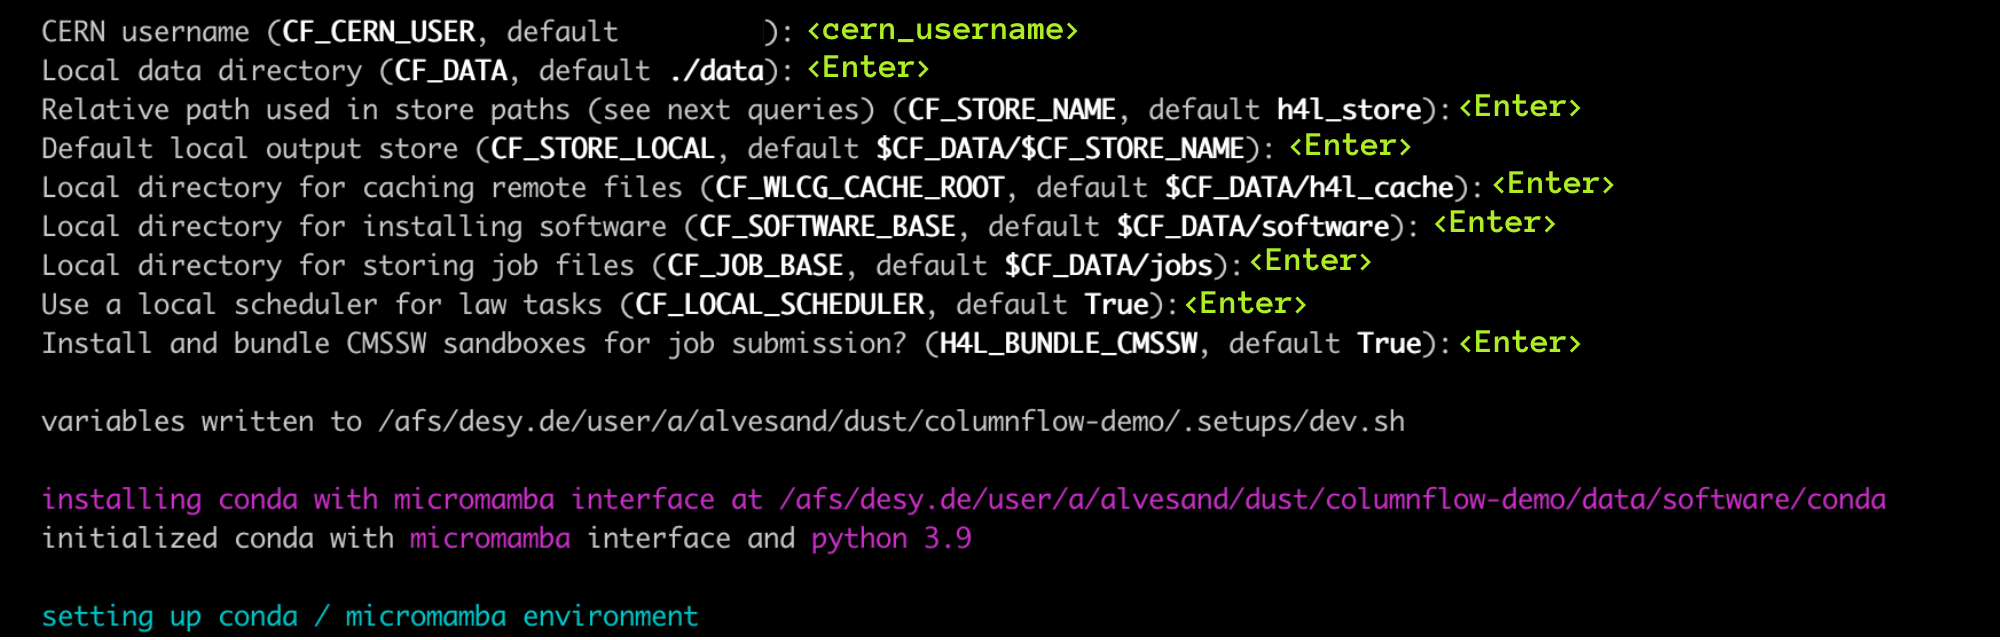
\includegraphics[scale=0.62]{images/setup.png}
\end{figure}

Note that the first installation of the software can take \underline{up to several minutes}.

Every time you want to work with ColumnFlow (e.g.\ if you open a new terminal window), you will need to source the \code{setup.sh} script again.

Once the installation is complete you should see a line of green text stating that the analysis has been successfully set up. You are now ready to start working with ColumnFlow!

\begin{figure}[!h]
    \centering
    \includegraphics[scale=0.62]{images/setup2.png}
\end{figure}

Inside of your newly created \code{columnflow-demo} directory, you will find the following project structure:
\begin{figure}[!h]
    \centering
    \includegraphics[scale=0.62]{images/CF_demo.png}
\end{figure}

%\subsection{ColumnFlow Tasks}

This exercise is organized in the form of \code{law} tasks, where different tasks create some form of output. You can view the available tasks by running:
\begin{lstlisting}[language=bash]
law index --verbose
\end{lstlisting}

This exercise will focus on the following tasks:

\begin{itemize}
    \item \texttt{\textcolor{LimeGreen}{cf.CalibrateEvents}} / \texttt{\textcolor{LimeGreen}{cf.SelectEvents}}
    \item \texttt{\textcolor{LimeGreen}{cf.ProduceColumns}}
    \item \texttt{\textcolor{LimeGreen}{cf.PlotCutflow}}
    \item \texttt{\textcolor{LimeGreen}{cf.PlotVariables1D}} / \texttt{\textcolor{LimeGreen}{cf.PlotVariables2D}}
    \item \texttt{\textcolor{LimeGreen}{cf.CreateDatacards}}
\end{itemize}

By default, these tasks will save their output on a remote file system (e.g.\ \texttt{WLGC}), for which you will require a \code{voms-proxy}. If you would like to save certain/all outputs locally, we recommend to create a directory on a system with a larger amount of disk space (e.g.\ \texttt{EOS}). For such cases, you will need to update the \code{law.cfg} file accordingly.


\section{Analysis strategy}

In order to find Higgs boson candidates, we need to reconstruct the four leptons in the final state. To select the four lepton candidates in the first place, we will need to write a \CCSPStlye{Selector} (Section~\ref{sec:selector}).

%, which will filter out all physics objects that do not fulfill the selection criteria. In this selector, we will implement \underline{kinematic cuts}, \underline{vertex cuts} and \underline{Isolation \& ID} criteria. We will also implement \underline{trigger selections} such that only events interesting for the $ZZ$ analysis are selected.

\begin{figure}[!h]
    \centering
    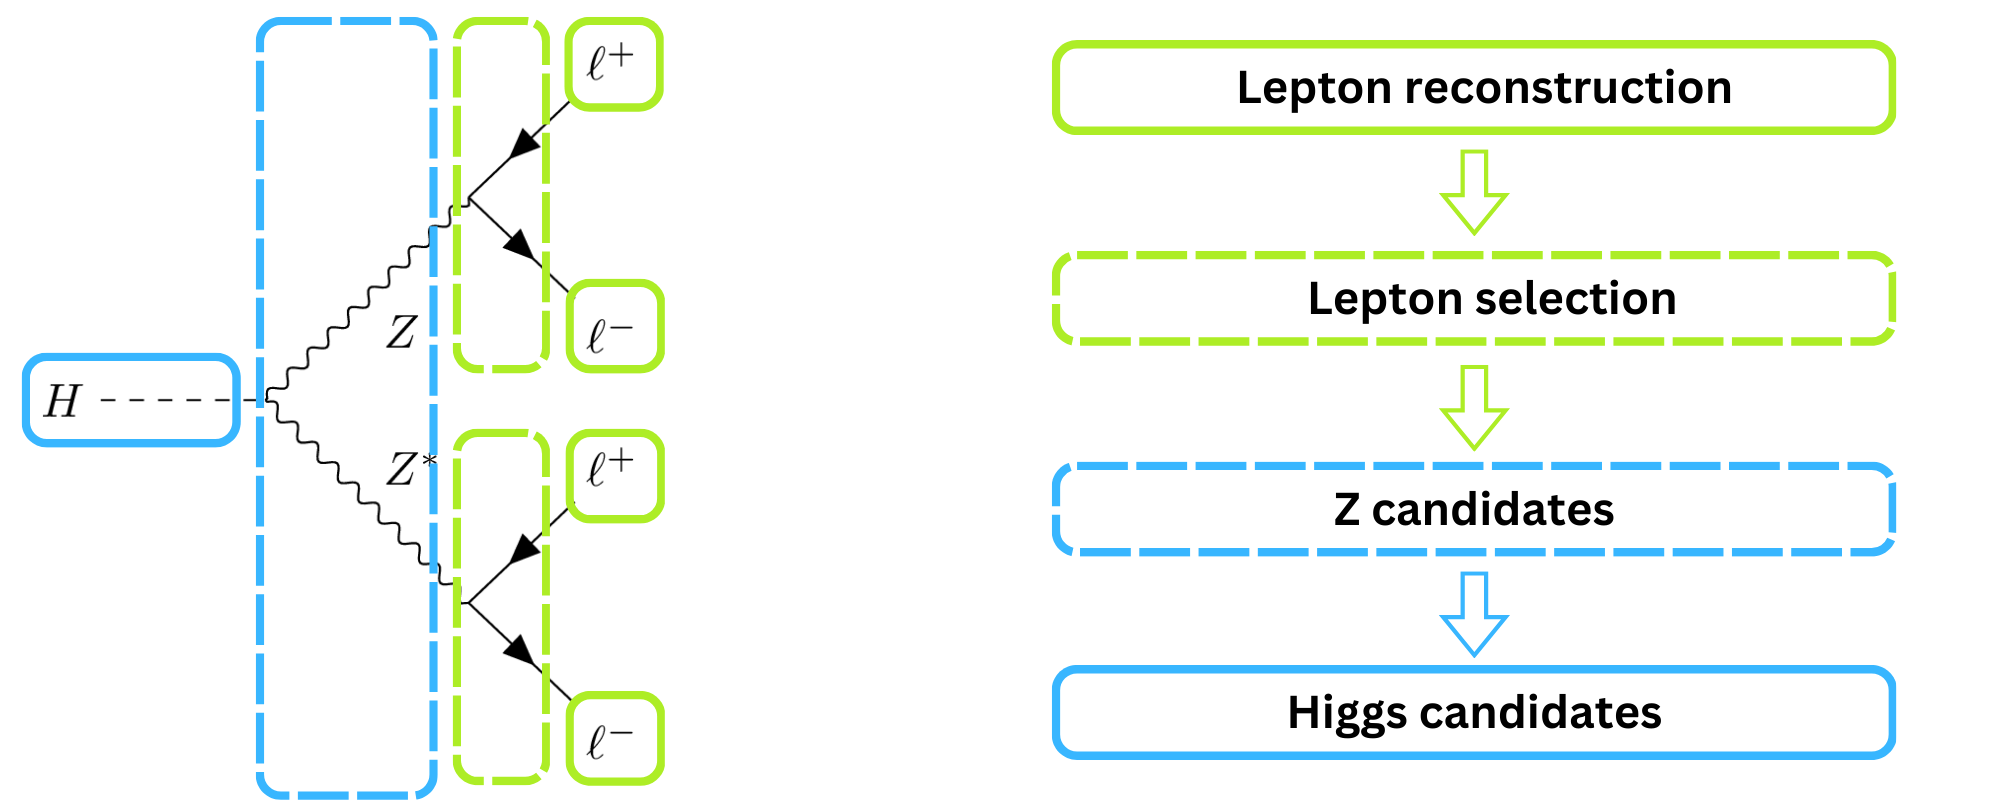
\includegraphics[scale=0.62]{images/strategy.png}
\end{figure}


    
\chapter{$H \rightarrow ZZ \rightarrow 4l$}
\justifying
\paragraph{}
The goal of this exercise is to reconstruct the Standard Model (SM) Higgs boson mass, using a selection targeting the four-lepton final state. This is considered a \textit{golden} channel to rediscovered the Higgs because:
\begin{itemize}
    \item there is a \textbf{\underline{ large signal to background ratio}} -- it is easy to discriminate between the peak of the reconstructed four-lepton mass ($m_{4l}$) and the overall flat background shape; 
    \item we have excellent \textbf{\underline{ mass resolution}} -- thanks to the great resolution power of CMS, we have optimal shape reconstruction of $m_{4l}$;
    \item it is a \textbf{\underline{ resolved final state}} -- detection of the four leptons in the final state ensures good discrimination of signal and background.
\end{itemize}

\begin{figure}[!h]
    \centering
    \includegraphics[scale=0.35]{images/plot.png}
    \caption{\justifying{Reconstructed four-lepton invariant mass $m_{4l}$ with 2018 data. The SM Higgs boson signal with $m_H = 125$ GeV, denoted as $H(125)$, and the $ZZ$ backgrounds are normalized to the SM expectation. The $Z+X$ background is normalized to the estimation from data.}}
    \label{higgs_plot}
\end{figure}

\section{Installation \& setup}
\justifying
\begin{tcolorbox}[colback=green!5!white,colframe=green!75!black,width=\textwidth]
Note: ColumnFlown only runs on Linux and may require up to 4 GB of disc space. \tcblower
Also, the machine where you run this exercise must be mounted with CERN AFS.
\end{tcolorbox}

Start by going to the GitLab repository of this exercise:

\texttt{\textcolor{LimeGreen}{\href{https://gitlab.cern.ch/cms-analysis/analysisexamples/columnflow-demo}{\underline{https://gitlab.cern.ch/cms-analysis/analysisexamples/columnflow-demo}}}}

To have your own copy of the code, fork the repository into your personal area. You can do this by clicking the \code{Fork} button on the upper right corner of the page. To set your Project URL please type your CERN username in the \code{Select a namespace} option.

\begin{figure}[!h]
    \centering
    \includegraphics[scale=0.62]{images/gitlab.png}
\end{figure}
\begin{figure}[!h]
    \centering
    \includegraphics[scale=0.62]{images/fork1.png}
\end{figure}

After clicking the \code{Fork project} button, your fork url should be:

\texttt{https://gitlab.cern.ch/<cern\_username>/columnflow-demo}

\newpage
In your forked project, go to the \code{Code} button on the right hand side of the page and copy the address under the \code{Clone with HTTPS} option. If you have an SSH key registered on GitLab prior to this exercise, you can also use the \code{Clone with SSH} option.

\begin{figure}[!h]
    \centering
    \includegraphics[scale=0.62]{images/fork2.png}
\end{figure}

Next, open a new terminal window and clone your code to your machine by running \underline{one of} the following commands (depending on which cloning method you chose):

\begin{lstlisting}[language=bash]
git clone --recursive https://gitlab.cern.ch/<cern_username>/columnflow-demo.git
\end{lstlisting}
\begin{lstlisting}[language=bash]
git clone --recursive ssh://git@gitlab.cern.ch:7999/<cern_username>/columnflow-demo.git
\end{lstlisting}

The directory you have thus created will be referred to as \code{basedir}. You can now go inside your local repository and install ColumnFlow. The \code{setup.sh} bash script will initialize the software environment with \code{micromamba}. Here, we define \code{dev} as the setup name, but you are free to name it as you wish.

\begin{lstlisting}[language=bash]
cd columnflow-demo
source setup.sh dev
\end{lstlisting}

You will be asked to define a series of variables, the first of which is your CERN username. For all other variables you can keep the default value by just pressing \code{Enter}. Variables specific to this exercise will start with \code{H4L\_}, while ColumnFlow specific variables start with \code{CF\_}. You can find all variables in the \code{.setups/dev.sh} bash file. We invite you to check out this file and familiarize yourself with these variables.

\begin{figure}[!h]
    \centering
    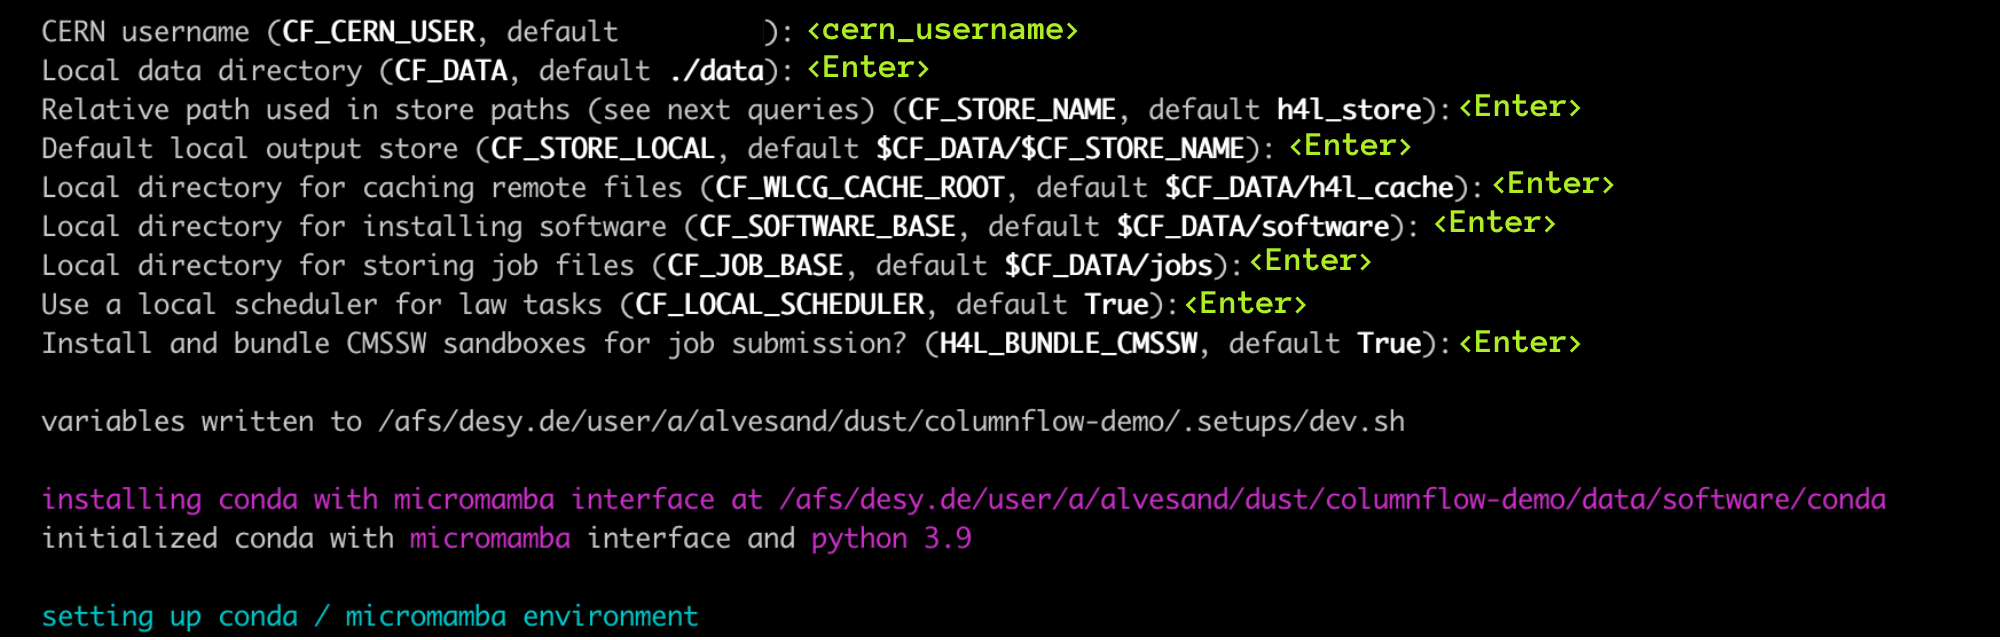
\includegraphics[scale=0.62]{images/setup.png}
\end{figure}

Note that the first installation of the software can take \underline{up to several minutes}.

Every time you want to work with ColumnFlow (e.g.\ if you open a new terminal window), you will need to source the \code{setup.sh} script again.

Once the installation is complete you should see a line of green text stating that the analysis has been successfully set up. You are now ready to start working with ColumnFlow!

\begin{figure}[!h]
    \centering
    \includegraphics[scale=0.62]{images/setup2.png}
\end{figure}

Inside of your newly created \code{columnflow-demo} directory, you will find the following project structure:
\begin{figure}[!h]
    \centering
    \includegraphics[scale=0.62]{images/CF_demo.png}
\end{figure}

%\subsection{ColumnFlow Tasks}

This exercise is organized in the form of \code{law} tasks, where different tasks create some form of output. You can view the available tasks by running:
\begin{lstlisting}[language=bash]
law index --verbose
\end{lstlisting}

This exercise will focus on the following tasks:

\begin{itemize}
    \item \texttt{\textcolor{LimeGreen}{cf.CalibrateEvents}} / \texttt{\textcolor{LimeGreen}{cf.SelectEvents}}
    \item \texttt{\textcolor{LimeGreen}{cf.ProduceColumns}}
    \item \texttt{\textcolor{LimeGreen}{cf.PlotCutflow}}
    \item \texttt{\textcolor{LimeGreen}{cf.PlotVariables1D}} / \texttt{\textcolor{LimeGreen}{cf.PlotVariables2D}}
    \item \texttt{\textcolor{LimeGreen}{cf.CreateDatacards}}
\end{itemize}

By default, these tasks will save their output on a remote file system (e.g.\ \texttt{WLGC}), for which you will require a \code{voms-proxy}. If you would like to save certain/all outputs locally, we recommend to create a directory on a system with a larger amount of disk space (e.g.\ \texttt{EOS}). For such cases, you will need to update the \code{law.cfg} file accordingly.


\section{Analysis strategy}

In order to find Higgs boson candidates, we need to reconstruct the four leptons in the final state. To select the four lepton candidates in the first place, we will need to write a \CCSPStlye{Selector} (Section~\ref{sec:selector}).

%, which will filter out all physics objects that do not fulfill the selection criteria. In this selector, we will implement \underline{kinematic cuts}, \underline{vertex cuts} and \underline{Isolation \& ID} criteria. We will also implement \underline{trigger selections} such that only events interesting for the $ZZ$ analysis are selected.

\begin{figure}[!h]
    \centering
    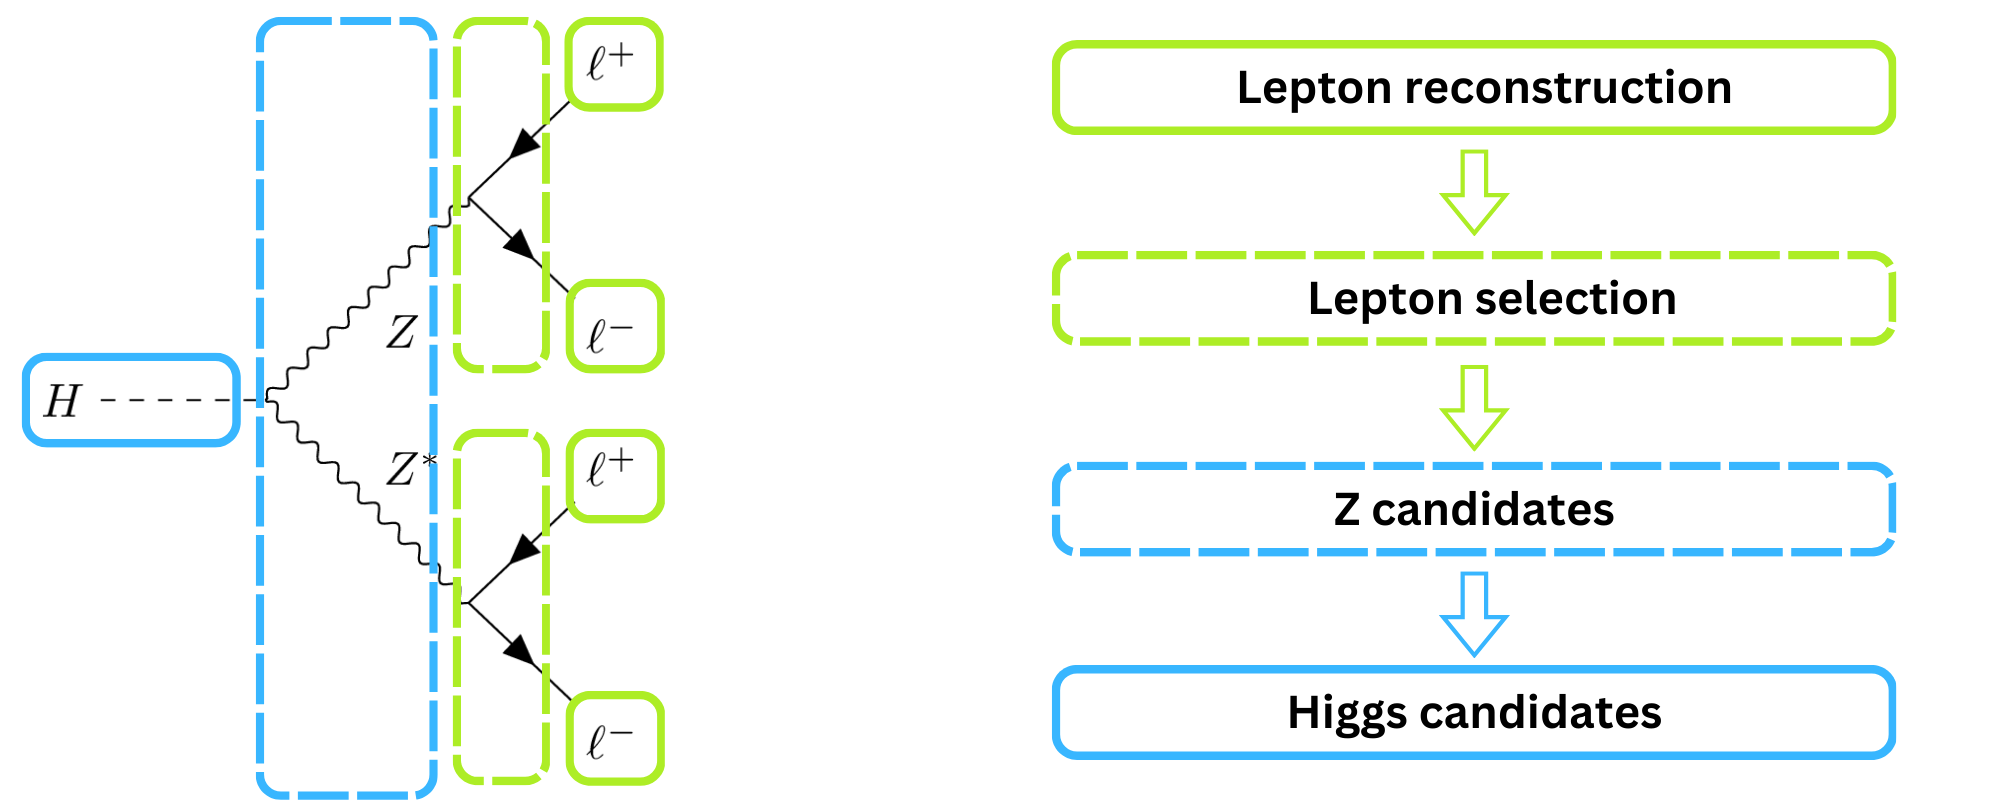
\includegraphics[scale=0.62]{images/strategy.png}
\end{figure}

\section{Writing a Calibrator}\label{sec:calibrator}
\section{Writing a Selector}\label{sec:selector}

The \CCSPStlye{Selector} class should be used to implement analysis selections.
This is a crucial step in the workflow since the decision to keep or reject objects or even whole events is performed here.
Since the selection usually depends on for example four-momenta of the objects within the events, it is executed after the calibration.
The corresponding task is called \CCSPStlye{cf.SelectEvents}.

For more information, please consider Ref.~\cite{cf_repo}.

\renewcommand{\arraystretch}{1.5}
\begin{table}[h!]
    \centering
    \begin{tabular}{|m{4cm}|m{5cm}|m{5.5cm}|}
    \hline
    & \textbf{Electrons} & \textbf{Muons} \\ \hline
    \textbf{Kinematic cuts} &
    \begin{itemize}[leftmargin=*]
    \item $p_T^e > 7$ GeV
    \item $|\eta^e| < 2.5$
    \end{itemize} &
    \begin{itemize}[leftmargin=*]
        \item $p_T^\mu > 5$ GeV
        \item $|\eta^\mu| < 2.5$
    \end{itemize} \\ \hline
    \textbf{Vertex cuts} &
    \begin{itemize}[leftmargin=*]
        \item $d_{xy} < 0.5$
        \item $d_z < 1$ cm
        \item $SIP < 4$
    \end{itemize} &
    \begin{itemize}[leftmargin=*]
        \item $d_{xy} < 0.5$
        \item $d_z < 1$ cm
        \item $SIP < 4$
    \end{itemize} \\ \hline
    \textbf{Isolation \& ID for \newline 'tight' working point} & Dedicated BDT targeting \newline prompt electrons. & Select only muons within \newline a well-defined cone ($R=0.35$). \\ \hline
    \end{tabular}
    \Caption{Selection criteria for leptons.}{Shown are the selection cuts for electrons/muons at the 'loose' working point, with the last row defining the extra requirement for the leptons to pass the 'tight' working point.}
    \label{leptonSelection}
\end{table}

In this part of the tutorial, we will write selections for electrons and muons.
In the script \code{h4l/selection/lepton.py} you can find the base structure to implement two \CCSPStlye{Selector} modules, \code{electron\_selection} and \code{muon\_selection}.
Each of these objects uses the relevant event information for its implementation.


\textbf{\underline{Electron Selection}}

For \code{electron\_selection}, the electron kinematic information is first loaded into the \code{uses} set.
Then, information that is dependent on the nanoAOD version is loaded. In this case, which MVA (Multi-Variate Analysis) flag should be used.
Notice that we use the union operator \code{|} to append either \code{Electron.mvaFall17V2Iso} or \code{Electron.mvaHZZIso} to the set containing the kinematic variables.
Lastly, to perform four-vector calculations, we also recquire \code{attach\_coffea\_behavior}, which is imported at the beginning of the script from \code{columnflow.selection.util}.


This \CCSPStlye{Selector} object also has two more dependencies, \code{exposed} and \code{sandbox}.
The first one determines whether or not the \CCSPStlye{Selector} object is available from the command line.
As mentioned in the last section, \code{sandbox} specifies the software enviorment where this \CCSPStlye{Selector} will be executed.

\newpage
\begin{itemize}
    \item {
        \textbf{\underline{Loose Electrons}} -- Within the main body of \code{electron\_selection}, all selections should be applied.
        Note that the minimum transverse momentum has already been specified in \code{min\_pt}.
        The actual value, in GeV, is set in \code{h4l/config/config\_h4l.py}, and depends on the argument \code{working\_point}.
        In the config file, a dictionary stores two possible values, $15$ for a \code{'tight'} working point (default value), and $7$ for a \code{'loose'} working point.
        Both the transverse momentum and the pseudorapidity selection criteria have already been applied in \code{default\_mask}.
        You should now complete the mask with the remaining selection criteria from Table \ref{leptonSelection}.
    }
    \item {
        \textbf{\underline{Tight Electrons}} -- Finally, you should also add a condition that applies the identification criteria for when \code{working\_point} is set to \code{'tight'}.
        Both the fSCeta and BDT values are set in the function \code{return\_electron\_id\_cuts}, which can be found in \code{h4l/selection/util.py}.
    }
\end{itemize}

After all selections have been applied, the final part of the module sorts all events by their momentum and applies the \code{default\_mask}.
The indices of selected events are then stored in \code{selected\_electron\_idx}.
The \code{electron\_selection} module finally returns both all events and a \CCSPStlye{SelectionResult} class instance.
We initiate the \CCSPStlye{SelectionResult} instance by setting the \code{objects} and \code{aux} (i.e. auxiliary) arguments.
Within \code{objects}, a nested dictionary saves \code{selected\_electron\_idx} as a value to an \code{Electron} key.
The selection mask itself, \code{default\_mask} is stored in \code{aux}.

\begin{exercise}{Writing a Selector -- Electron Selection}[h4l/selection/lepton\_solution.py]
	Refering to Table \ref{leptonSelection}, fill in the missing information in the \CCSPStlye{Selector} module \code{electron\_selection} defined in \code{h4l/selection/lepton.py}.
\end{exercise}

\vspace{0.8cm}

\textbf{\underline{Muon Selection}}

The \code{muon\_selection} module behaves very similarly. In this case, a dedicated software environment is not required.
There is also no information dependent on the nanoAOD version.
Besides the kinematic information, the \code{uses} set also loads muon quality criteria (e.g. if it is a global or tracker muon), identification and isolation information.

\begin{itemize}
    \item {
        \textbf{\underline{Loose Muons}} -- Within the main body of \code{muon\_selection}, a selection mask is now defined \code{selected\_muon\_mask}.
        Similarly to the electron selection, the minimum transverse momentum and pseudorapidity are already defined.
        You should now expand this mask such that:
        \begin{enumerate}
            \item you recquire either a global or tracker muon (for tracker muons \code{nStations} should be a positive);
            \item discard standalone muon if the reconstructed tracks are only present in the muon system (i.e. for standalone muons, you should recquire a positive number of \code{nTrackerLayers});
            \item apply the remaining selection criteria from Table \ref{leptonSelection}.
        \end{enumerate}
    }
    \item {
        \textbf{\underline{Tight Muons}} -- You should now add three conditions to \code{selected\_muon\_mask}:
        \begin{enumerate}
            \item enforce that the low momentum muons ($< 200$ GeV) are ParticleFlow candidates (use the variable \code{isPFcand});
            \item enforce that the high momentum muons ($\geq 200$ GeV) are ParticleFlow candidates OR have a positive \code{highPtId};
            \item use the variable \code{pfRelIso03\_all} to apply the condition in Table \ref{leptonSelection}.
        \end{enumerate}
    }
\end{itemize}

\begin{exercise}{Writing a Selector -- Muon Selection}[h4l/selection/lepton\_solution.py]
	Again refering to Table \ref{leptonSelection}, fill in the missing information in the \CCSPStlye{Selector} module \code{muon\_selection} defined in \code{h4l/selection/lepton.py}.
\end{exercise}

    
\chapter{Advanced Topics}\label{chap:advanced}

\chapter{Advanced Topics}\label{chap:advanced}
\section{Defining categories}\label{sec:categories}

\section{Defining Systematic Uncertainties}\label{sec:shifts}
\section{Define Sets of Weights to use for Templates}\label{sec:event_weights}
\section{Writing datacards}\label{sec:inference}


\appendix
\printbibliography

\end{document}
